\subsection{セットアップ}
次に,Himeoka and Kaneko (2017)のモデル\cite{hk17}を参考に,代謝物Xを生成する反応が失敗しうるモデルを考えた.
まず,代謝物Xを作る反応において,ある確率$\epsilon$でエラーが発生し,ゴミ分子Zができると仮定する.
さらに,ゴミ分子Zは代謝物Xと可逆的に結合し,複合体Cを作ると仮定する.
これは,代謝物Xの自己触媒を阻害する反応である.
つまり,以下の拡散および反応を考える:
\begin{align}
  \ce{N &<->[$D$] Y} \\
  \ce{Y + X &->[$k(1-\epsilon)$] X + X} \\
  \ce{Y + X &->[$k\epsilon$] Z + X} \\
  \ce{Z + X &<=>[$k_1$][$k_2$] C} \\
  \ce{X &->[\phi] \emptyset}.
\end{align}
よって,化学種X,Y,Z,Cの濃度をそれぞれ$x,y,z,c$とおくと,方程式は次のようになる:
\begin{align}
  \frac{dx}{dt} &= k(1-\epsilon)xy - k_1 xz + k_2 c - \phi x - \mu x\\
  \frac{dy}{dt} &= D(n-y) - kxy - \mu y \\
  \frac{dz}{dt} &= k\epsilon xy - k_1 xz + k_2 c - \mu z \\
  \frac{dc}{dt} &= k_1 xz - k_2 c - \mu c \\ 
  \mu &= \gamma \phi x.
\end{align}

\subsection{結果と考察}
\subsubsection{エラー率が一定の場合}
まず,$\epsilon$が定数である場合を考える.
このとき,成長条件は$n > n^* = \phi/(k(1-\epsilon))$であることが次のように示せる.

まず,微分方程式で$d/dt=0$として得られる代数方程式から
\begin{align}
  y &= \frac{n}{1+\frac{k+\gamma\phi}{D}x} \\
  c &= \frac{k_1xz}{k_2+\gamma\phi x}
\end{align}
が導かれる.
これを用いて,同様に得られる残り2本の代数方程式から$c$を消去すると,$x\neq 0$なる定常解に対して
\begin{align}
  z &= \frac{\phi(1+\gamma x) - k(1-\epsilon)y}{\frac{k_1k_2}{k_2+\gamma\phi x} - k_1} \\
  z &= \frac{-k\epsilon y}{\frac{k_1k_2}{k_2+\gamma\phi x} - k_1 - \gamma\phi}
\end{align}
がそれぞれ導かれる.
さらに,この二つが等しいとした式から$y$を消去することで,Xの濃度$x$の0以外の定常解は
\begin{equation}
  1-\epsilon \left[1 + \left(\frac{k_2}{k_1 x} + 1 - \frac{\gamma \phi}{k_1}\right)^{-1} \right] = \frac{\phi}{kn}(1+\gamma x)\left(1+\frac{k+\gamma\phi}{D}x\right)
\end{equation}
を満たすと分かる.
さらに$x \ge 0$において,左辺は$x$とともに減少し,右辺は$x$とともに増加することから,定常解$x>0$が存在する条件は,
\begin{equation}
  1-\epsilon > \frac{\phi}{kn}
\end{equation}
と分かる.
したがって,栄養濃度の満たすべき条件は
\begin{equation}
  n > n^* = \frac{\phi}{k(1-\epsilon)} \label{nast_errconst}
\end{equation}
と求まる.

この式は,代謝物Xの消費反応の速度定数が$\phi$,生成反応の実効的な速度定数が$k(1-\epsilon)$となることから説明できる.
また,反応$\ce{Z + X <=> C}$はここでは効いていないことが分かる.

しかし,この証明のような解析的な手法では,式\eqref{nast_errconst}が成り立つときに$x>0$を満たす定常解が安定であること(成長速度が正の値で安定すること)を示すのが難しかった.
そこで次に,数値計算によって式\eqref{nast_errconst}と成長速度が正であることが等価であることを部分的に確認した.
ここでは,パラメータ$k,k_1,k_2,\phi,\gamma,D$はすべて1とした.
まず,外部栄養濃度$n$をある値に固定し,$\epsilon=0,0.2,0.4,0.6,0.8$のそれぞれについて,初期濃度を$x=y=1, z=c=0$として十分な時間(時刻$t=10^5$まで)シミュレーションを行った.
その結果,最終的にすべての成分濃度と成長速度$\mu$が定常となっていることを確認した.
このとき,外部栄養濃度$n$と定常成長速度$\mu$の関係は図\ref{fig:n_vs_mu_errconst}のようになった.
この図を参考に,定常成長速度が$\mu > 10^{-3}$となる最小の外部栄養濃度$n^*$を「成長に必要な栄養濃度」と考えることにした.
そこで,外部栄養濃度$n$を0から0.1ずつ増加させ,$\mu>10^{-3}$となる最小の$n$を$n^*$として,$\epsilon$と$n^*$の関係をプロットした(図\ref{fig:err_vs_n_errconst}).
この図から,理論式\eqref{nast_errconst}はこの数値計算の結果と整合することが確認できる.

\begin{figure}[htbp]
  \centering
  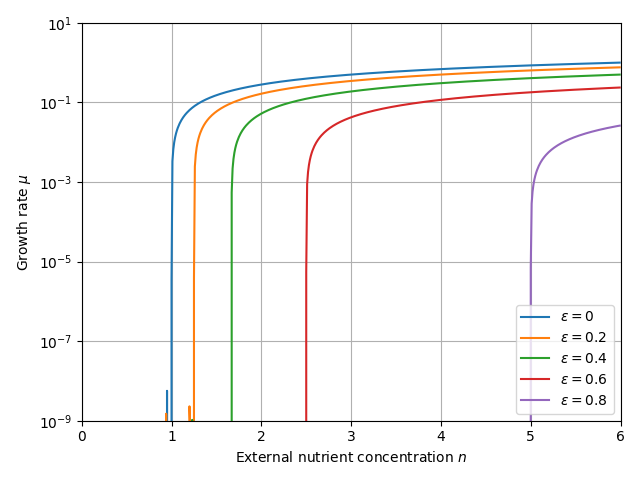
\includegraphics[width=10cm]{n_vs_mu_errconst.png}
  \caption{エラー率を定数($\epsilon=0,0.2,0.4,0.6,0.8$)として計算した,時刻$t=10^5$における外部栄養濃度$n$と成長速度$\mu$の関係(初期濃度は$x=y=1, z=c=0$,時間の刻み幅は0.1,$n$の刻み幅は0.01,その他のパラメータ$k,k_1,k_2,\phi,\gamma,D$はすべて1とした.).この結果は式\eqref{nast_errconst}と整合する.}
  \label{fig:n_vs_mu_errconst}
\end{figure}

\begin{figure}[htbp]
  \centering
  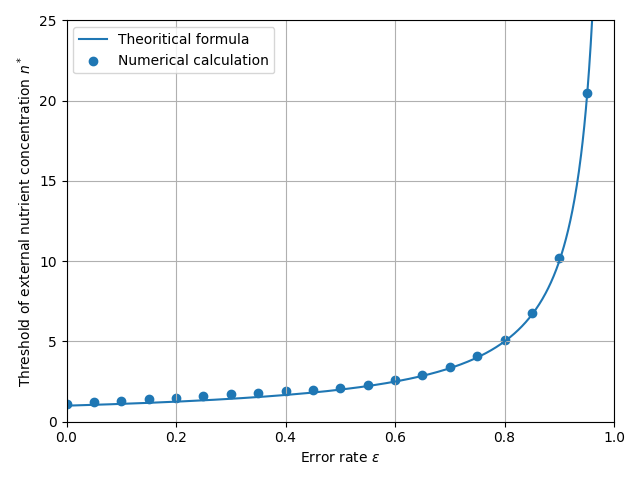
\includegraphics[width=10cm]{err_vs_n_errconst.png}
  \caption{エラー率が定数であるとして計算した,$\epsilon$と成長に必要な($\mu > 10^{-3}$となる最小の)外部栄養濃度$n^*$の関係(Numerical calculationとして示したプロット.$n^*$を求めるにあたって,$n$は刻み幅0.1で変更した.それ以外のパラメータは図\ref{fig:n_vs_mu_errconst}と同様である.).これは式\eqref{nast_errconst}で表される理論線(Theoritical formulaとして示した曲線)と整合している.}
  \label{fig:err_vs_n_errconst}
\end{figure}

\subsubsection{エラー率が代謝物濃度$x$に依存する場合}
次に,エラー率$\epsilon$が変化する場合を考える.
まず,ここでは代謝物濃度$x$に依存して
\begin{equation}
  \epsilon = \frac{\delta}{K + x} \label{errx}
\end{equation}
と書ける場合を考える.
ただし,エラー率は0以上1以下の値をとるので,$0 \le \delta \le K$とする.
なお,この式の形は,Himeoka and Kaneko (2017)のモデル\cite{hk17}を参考に,代謝物Xが多いときにエラー率が低くなるようにした.

この場合には,解析的に定常解を求めることがやや困難なので,数値計算の結果をもとに考察を行う.

まず,$K=1$とし,$\delta=0,0.2,0.4,0.6,0.8,1$のそれぞれについて,先ほどと同様にシミュレーションを行った.
その結果,外部栄養濃度$n$と定常成長速度$\mu$の関係は図\ref{fig:n_vs_mu_K1s0}のようになった.
この図を参考に,定常成長速度が$\mu > 10^{-3}$となる最小の外部栄養濃度$n^*$を「成長に必要な栄養濃度」と考えた.
そして,$K=0.1,0.5,1$のそれぞれについて,$\delta/K$と$n^*$の関係をプロットした(図\ref{fig:err_vs_n_errslope_s0}).
また,同図に$\epsilon=\delta/K$で一定としたときの理論線(式\eqref{nast_errconst})も記載した.
これらを比較すると,$\delta/K$が小さいときのプロットは理論線と重なっているが,$\delta/K$が大きいときは理論線とずれて,$n^*$が発散しなくなることが分かった.
また,理論線から外れ始める$\delta/K$の値は,$K$とともに増加することも分かった.

次にその理由を考察する.
まず$\delta/K$が小さいとき,エラー率が低いため$n^*$は小さく済む.
これに伴い,$n\approx n^*$において$x \ll K$が成り立つ.
(いま,$\gamma=\phi=1$として計算しているので,$\mu=x$が成り立つ.つまりこの主張は,図\ref{fig:n_vs_mu_K1s0}の縦軸を,$n\approx n^*$におけるXの濃度$x$と読み替えることで確認できる.)
そのため,式\eqref{errx}より$\epsilon \approx \delta/K$と考えて良い.
よって,エラー率が$\delta/K$で一定と考えた場合と結果が一致すると考えられる.
逆に,$\delta/K$が大きいとき,$x$が$K$に対して無視できず,$x$が大きいほどエラー率が$\delta/K$よりも小さくなることで,$n^*$が小さく済むと考えられる.
さらに,$K$が大きい方が$x \ll K$となりやすいので,$\epsilon=\delta/K$の曲線から外れづらくなると説明できる.

\begin{figure}[htbp]
  \centering
  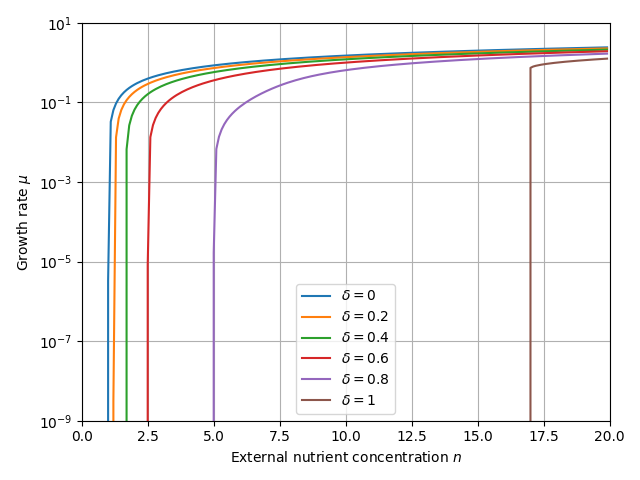
\includegraphics[width=10cm]{n_vs_mu_K1s0_errslope_all.png}
  \caption{エラー率が$x$に式\eqref{errx}の形($K=1$,$\delta=0,0.2,0.4,0.6,0.8,1$)で依存するとして計算した,時刻$t=10^5$における外部栄養濃度$n$と成長速度$\mu$の関係($n$の刻み幅を0.1に変更した.それ以外のパラメータは図\ref{fig:n_vs_mu_errconst}と同様である.).この結果を見ると,$\delta=1$以外は,$\epsilon=\delta/K$とみなしたときの図\ref{fig:n_vs_mu_errconst}と変わらないことが分かる.}
  \label{fig:n_vs_mu_K1s0}
\end{figure}

\begin{figure}[htbp]
  \centering
  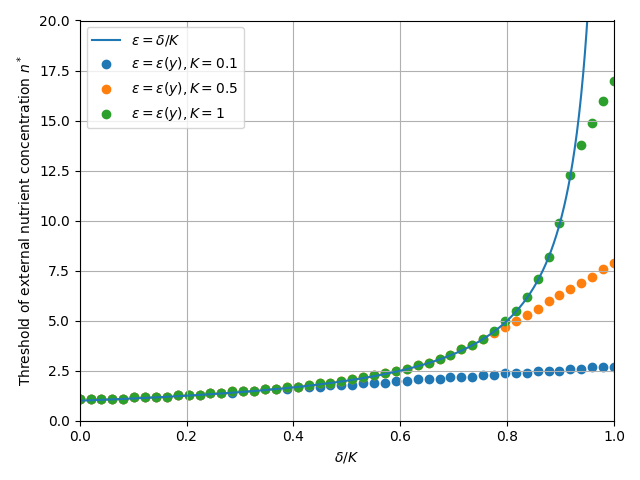
\includegraphics[width=10cm]{err_vs_n_errslope_s0_K.png}
  \caption{エラー率が$x$に式\eqref{errx}の形($K=0.1,0.5,1$)で依存するとして計算した,$\delta$と成長に必要な($\mu > 10^{-3}$となる最小の)外部栄養濃度$n^*$の関係($n$は刻み幅0.1で変更した.それ以外のパラメータは図\ref{fig:n_vs_mu_errconst}と同様である.).これを$\epsilon=\delta/K$のときの理論線と比較すると,$\delta/K$が大きくなるにつれて差が広がることが分かる.また,プロットが理論線から外れ始める$\delta/K$の値は,$K$とともに増加する.}
  \label{fig:err_vs_n_errslope_s0}
\end{figure}

\subsubsection{エラー率が内部栄養濃度$y$に依存する場合}
次に,エラー率が細胞内の栄養濃度$y$に依存して
\begin{equation}
  \epsilon = \frac{\delta}{K + y} \label{erry}
\end{equation}
と書ける場合を考える.
この場合に,$K=1$として同様の数値計算を行い,$\delta$と定常成長速度$\mu$の関係をプロットした(図\ref{fig:n_vs_mu_K1s1}).
次に,この図を参考に,成長に必要な外部栄養濃度$n^*$をこれまでとまったく同じように定義した.
そして,$K=1,10,100$のそれぞれについて,$\delta/K$と$n^*$の関係をプロットした(図\ref{fig:err_vs_n_errslope_s1}).
この図からも,図\ref{fig:err_vs_n_errslope_s0}と同じく,$\delta/K$が大きくなると理論線(式\eqref{nast_errconst}で$\epsilon=\delta/K$としたもの)から外れることと,$K$が大きいとプロットが理論線から外れ始める$\delta/K$の値が大きくなることが読み取れる.
それらについての考察は同様なので省略する.

一方で,図\ref{fig:err_vs_n_errslope_s0}と図\ref{fig:err_vs_n_errslope_s1}を比べると,同じ$K$の値に対し,エラー率が$x$に依存しているときに比べて,$y$に依存しているときの方が$n^*$が小さく済むことが読み取れる.
これについては,以下のように説明ができる.
まず,成長できる最小限近くの外部栄養濃度$n\approx n^*$において,$\mu$が小さいことから$x$は小さい.
その一方で,$y$は拡散流入により$n^*$近くの値になる.
つまり,$x$より$y$の方が大きいため,エラー率は式\eqref{errx}よりも式\eqref{erry}の方が小さくなる.
その結果,エラー率が$y$に依存する場合の方が$n^*$が少なく済むと考えられる.

\begin{figure}[htbp]
  \centering
  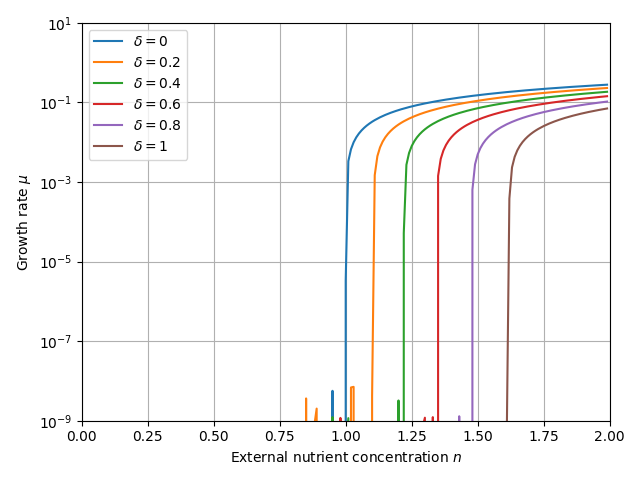
\includegraphics[width=10cm]{n_vs_mu_K1s1_errslope.png}
  \caption{エラー率が$y$に式\eqref{erry}の形($K=1$,$\delta=0,0.2,0.4,0.6,0.8,1$)で依存するとして計算した,時刻$t=10^5$における外部栄養濃度$n$と成長速度$\mu$の関係(刻み幅,初期濃度,パラメータの取り方は図\ref{fig:n_vs_mu_errconst}のときと同様である.).この場合,エラー率が$x$依存する場合と比べて,成長に必要な$n$は少なく済む.}
  \label{fig:n_vs_mu_K1s1}
\end{figure}

\begin{figure}[htbp]
  \centering
  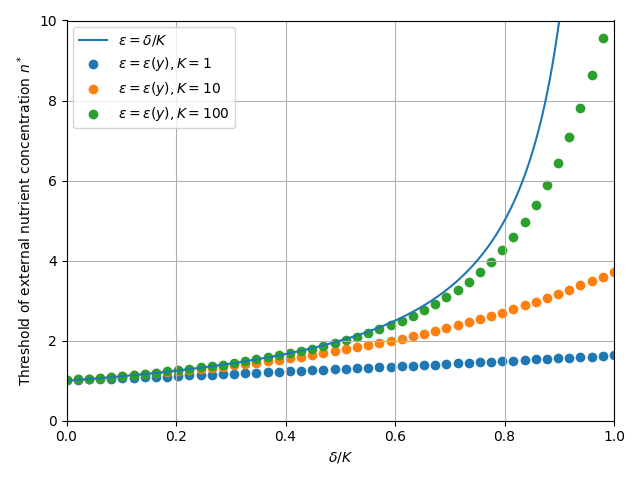
\includegraphics[width=10cm]{err_vs_n_errslope_s1_K.png}
  \caption{エラー率が$y$に式\eqref{erry}の形($K=1,10,100$)で依存するとして計算した,$\delta$と成長に必要な($\mu > 10^{-3}$となる最小の)外部栄養濃度$n^*$の関係($n$は刻み幅0.01で変更した.それ以外のパラメータは図\ref{fig:n_vs_mu_errconst}と同様である.).}
  \label{fig:err_vs_n_errslope_s1}
\end{figure}

